\documentclass{urdpl}     % praca w języku polskim

% Lista wszystkich języków stanowiących języki pozycji bibliograficznych użytych w pracy.
% (Zgodnie z zasadami tworzenia bibliografii każda pozycja powinna zostać utworzona zgodnie z zasadami języka, w którym dana publikacja została napisana.)
\usepackage[english,polish]{babel}

% Użyj polskiego łamania wyrazów (zamiast domyślnego angielskiego).
\usepackage{polski}

\usepackage[utf8]{inputenc}

% dodatkowe pakiety

\usepackage{mathtools}
\usepackage{amsfonts}
\usepackage{amsmath}
\usepackage{amsthm}
\usepackage[hidelinks]{hyperref}
\usepackage{float}
\usepackage{listings}
\usepackage{graphicx}
\usepackage{subcaption}
\usepackage{booktabs} % Dla \toprule, \midrule, \bottomrule
\usepackage{multirow} 
\usepackage{tabularx} 
\usepackage{amssymb} 
\usepackage{listings}
\usepackage{xcolor}
\usepackage{array}
\usepackage{makecell}
\usepackage[flushleft]{threeparttable}
\usepackage[normalem]{ulem}
\usepackage{lineno}
% ---------------------------------------------

% --- < bibliografia > ---

\usepackage{csquotes}

% ------------------------
% --- < listingi > ---

% Użyj czcionki kroju Courier.
\usepackage{courier}

\usepackage{listings}
\lstloadlanguages{TeX}
\renewcommand{\lstlistlistingname}{Spis listingów}
\renewcommand{\lstlistingname}{Listing}


\lstset{
	literate={ą}{{\k{a}}}1
           {ć}{{\'c}}1
           {ę}{{\k{e}}}1
           {ó}{{\'o}}1
           {ń}{{\'n}}1
           {ł}{{\l{}}}1
           {ś}{{\'s}}1
           {ź}{{\'z}}1
           {ż}{{\.z}}1
           {Ą}{{\k{A}}}1
           {Ć}{{\'C}}1
           {Ę}{{\k{E}}}1
           {Ó}{{\'O}}1
           {Ń}{{\'N}}1
           {Ł}{{\L{}}}1
           {Ś}{{\'S}}1
           {Ź}{{\'Z}}1
           {Ż}{{\.Z}}1,
	basicstyle=\footnotesize\ttfamily,
}

% defninicja stylu python
\lstdefinestyle{stylePython}{
    language=Python,
    commentstyle=\color{green},          % Kolor komentarzy
    keywordstyle=\color{blue},           % Kolor słów kluczowych
    numberstyle=\tiny\color{gray},       % Kolor i styl numerów linii
    stringstyle=\color{red},             % Kolor ciągów znaków
    basicstyle=\ttfamily\footnotesize,   % Podstawowy styl kodu
    breakatwhitespace=false,             % Automatyczne dzielenie wierszy
    breaklines=true,                     % Dzielenie długich linii
    keepspaces=true,                     % Zachowanie spacji
    numbers=left,                        % Numery linii po lewej
    numbersep=5pt,                       % Odstęp numerów od kodu
    showspaces=false,                    % Nie pokazuj spacji
    showstringspaces=false,              % Nie pokazuj spacji w ciągach znaków
    showtabs=false,                      % Nie pokazuj tabulacji
    tabsize=2                            % Rozmiar tabulacji
}

% defnicja stylu JAVA
\lstdefinestyle{javaStyle}{
    language=Java,
    basicstyle=\ttfamily\footnotesize,
    keywordstyle=\color{blue},
    commentstyle=\color{green!50!black}\itshape,
    stringstyle=\color{green},
    numberstyle=\tiny\color{gray},
    numbers=left,
    numbersep=5pt,                       % Odstęp numerów od kodu
    stepnumber=1,
    showspaces=false,                    % Nie pokazuj spacji
    tabsize=2,
    showstringspaces=false,
    breaklines=true,
    breakatwhitespace=false,             % Automatyczne dzielenie wierszy
    showtabs=false,                      % Nie pokazuj tabulacji
    keepspaces=true                    % Zachowanie spacji
}


\definecolor{stringcolor}{RGB}{163,21,21}    % pomarańczowy - stringi
\definecolor{typecolor}{RGB}{43, 145, 176}     % ciemny fiolet - klasy, typy

\lstdefinestyle{csStyle}{
    language=[Sharp]C, % dla C#; można zmienić na Java
    basicstyle=\ttfamily\footnotesize,
    keywordstyle=\color{blue},
    stringstyle=\color{stringcolor},
    commentstyle=\color{green!50!black}\itshape,
    morekeywords={class, public, private, protected, static, void, string, int, new}, % dodatkowe słowa kluczowe
    emphstyle=\color{typecolor}\bfseries, % klasy na fioletowo
    numbers=left,
    numbersep=5pt,                       % Odstęp numerów od kodu
    numberstyle=\tiny\color{gray},
    stepnumber=1,
    breaklines=true,
    showspaces=false,                    % Nie pokazuj spacji
    tabsize=2,
    showstringspaces=false,
    breakatwhitespace=false,             % Automatyczne dzielenie wierszy
    showtabs=false,                      % Nie pokazuj tabulacji
    keepspaces=true                    % Zachowanie spacji  
}

\definecolor{lightgray}{rgb}{0.9,0.9,0.9}
    % \definecolor{blue}{rgb}{0,0,1}
    \definecolor{green}{rgb}{0,0.6,0}
    % \definecolor{red}{rgb}{0.6,0,0}
    \definecolor{gray}{rgb}{0.5,0.5,0.5}

% % ------------------------
\AtBeginDocument{
	\renewcommand{\tablename}{Tabela}
	\renewcommand{\figurename}{Rys.}   
    \newcommand{\listingname}{Listing}
}


% ------------------------
% --- < tabele > ---

% defines the X column to use m (\parbox[c]) instead of p (`parbox[t]`)
\newcolumntype{C}[1]{>{\hsize=#1\hsize\centering\arraybackslash}X}

%---------------------------------------------------------------------------

\author{Mykhailo Kleban}
\shortauthor{M. Kleban}
\noAlbum{134922}

\titlePL{System rezerwacji sal/podział godzin}
\titleEN{Thesis in \LaTeX}

\shorttitlePL{Przygotowanie dokumentacji do projektu w~systemie~\LaTeX} % skrócona wersja tytułu jeśli jest bardzo długi
\shorttitleEN{Preparation of a long and fascinating thesis in \LaTeX}

\thesistype{Praca projektowa}


\thesisDone{Praca wykonana pod kierunkiem}
\supervisor{dr inż. Ewa Żesławska}
%\supervisor{Jan Nowak PhD}

\degreeprogramme{Informatyka}
%\degreeprogramme{Computer Science}

\date{2025}

\department{Instytut Informatyki}
%\department{Institute of Computer Science}

\faculty{Wydział Nauk Ścisłych i Technicznych}
%\faculty{Faculty of Science and Technology}



\setlength{\cftsecnumwidth}{10mm}

%---------------------------------------------------------------------------
\setcounter{secnumdepth}{4}
\brokenpenalty=10000\relax

% --------------------------------------------------------------------------
% główna część pracy
% --------------------------------------------------------------------------

\begin{document}

\titlepages

% Ponowne zdefiniowanie stylu `plain`, aby usunąć numer strony z pierwszej strony spisu treści i poszczególnych rozdziałów.
\fancypagestyle{plain}
{
    % Usuń nagłówek i stopkę
    \fancyhf{}
    % Usuń linie.
    \renewcommand{\headrulewidth}{0pt}
    \renewcommand{\footrulewidth}{0pt}
}

\setcounter{tocdepth}{2}
\tableofcontents
\clearpage


% dodanie poszczególnych rozdziałów 

\chapter{Wstęp}

\section{Cel projektu}

Celem projektu było zaprojektowanie i zaimplementowanie aplikacji desktopowej wspomagającej zarządzanie zajęciami akademickimi oraz rezerwację sal dydaktycznych w środowisku uczelni wyższej.  
System ma za zadanie ułatwić pracownikom sekretariatu organizację planów zajęć, eliminując problemy związane z ręcznym układaniem grafiku.

\section{Zakres funkcjonalny systemu}

Dzięki zastosowanym funkcjonalnościom możliwe jest m.in.:
\begin{itemize}
    \item dodawanie nowych zajęć do bazy danych,
    \item filtrowanie według różnych kryteriów (typ, sala, grupa),
    \item edytowanie istniejących rekordów,
    \item sprawdzanie dostępności sal i konfliktów czasowych.
\end{itemize}

Aplikacja automatycznie weryfikuje poprawność danych wejściowych oraz wyświetla komunikaty błędów w przypadku wykrycia kolizji.

\section{Zastosowane technologie}

Projekt został zrealizowany w języku \textbf{Java}, przy użyciu biblioteki \textbf{Swing} do stworzenia graficznego interfejsu użytkownika.  
Do komunikacji z bazą danych zastosowano technologię \textbf{JDBC}, natomiast dane przechowywane są w relacyjnej bazie danych \textbf{PostgreSQL}.

\section{Struktura dokumentacji}

Dokumentacja została przygotowana z użyciem systemu składu tekstu \LaTeX{} i zawiera:
\begin{itemize}
    \item opis struktury aplikacji,
    \item diagramy klas i bazy danych,
    \item opis interfejsu użytkownika,
    \item opis komponentów i funkcjonalności systemu.
\end{itemize}

\chapter{Opis projektu}

\section{Cel i przeznaczenie}

Projekt \textbf{System rezerwacji sal / podział godzin} został zaprojektowany z myślą o ułatwieniu zarządzania harmonogramem zajęć akademickich.  
Głównym celem systemu jest wsparcie administracji uczelni w planowaniu i koordynowaniu zajęć dydaktycznych w sposób zautomatyzowany i intuicyjny.

\section{Główne funkcjonalności}

System umożliwia użytkownikowi wykonywanie następujących operacji:

\begin{itemize}
    \item dodawanie zajęć wraz z informacjami: dzień tygodnia, godzina, typ zajęć, kierunek, przedmiot, prowadzący, sala, grupa;
    \item edytowanie oraz usuwanie wcześniej dodanych zajęć;
    \item filtrowanie zajęć według sali, grupy i typu zajęć;
    \item walidację danych przy wprowadzaniu (np. sprawdzanie konfliktów sal i grup);
    \item obsługę wyjątków i prezentację komunikatów błędów.
\end{itemize}

\section{Typy zajęć}

System rozróżnia trzy typy zajęć, które różnią się liczbą przypisanych grup:

\begin{itemize}
    \item \textbf{Wykład (Wyklad)} – przeznaczony dla wszystkich grup;
    \item \textbf{Projekt (ćwiczenia)} – przeznaczony dla dwóch konkretnych grup (np. A i B);
    \item \textbf{Laboratorium} – przeznaczone dla jednej grupy.
\end{itemize}

\section{Zastosowane technologie}

Do realizacji projektu wykorzystano następujące technologie:

\begin{itemize}
    \item język \textbf{Java}, którego zasady zostały zaczerpnięte z literatury \cite{horstmann};
    \item biblioteka \textbf{Swing} do budowy graficznego interfejsu użytkownika;
    \item baza danych \textbf{PostgreSQL};
    \item interfejs \textbf{JDBC} do komunikacji z bazą danych;
    \item wzorzec projektowy \textit{DAO}, zgodnie z podejściem przedstawionym w \cite{dao}.
\end{itemize}

\chapter{Implementacja systemu}

System został zaimplementowany w języku \textbf{Java}, z wykorzystaniem biblioteki \textbf{Swing} do budowy graficznego interfejsu użytkownika oraz technologii \textbf{JDBC} do komunikacji z bazą danych \textbf{PostgreSQL}.

\section{Struktura aplikacji}

Struktura projektu została logicznie podzielona na pakiety zgodnie z zasadami dobrej organizacji kodu. W folderze \texttt{src} znajdują się wszystkie elementy źródłowe aplikacji, zorganizowane w następujący sposób:

\begin{itemize}
    \item \texttt{dao} – klasy odpowiedzialne za dostęp do danych:
    \begin{itemize}
        \item \texttt{LoginDAO} – obsługa uwierzytelniania użytkownika;
        \item \texttt{ZajeciaDAO} – operacje CRUD na tabeli zajęć.
    \end{itemize}

    \item \texttt{database} – logika połączenia z bazą danych:
    \begin{itemize}
        \item \texttt{DatabaseConnection} – klasa łącząca aplikację z PostgreSQL.
    \end{itemize}

    \item \texttt{DodajZajeciaPanel} – komponent GUI odpowiedzialny za dodawanie nowych zajęć:
    \begin{itemize}
        \item \texttt{DodajZajeciaPanel.java/.form} – panel formularza oraz jego widok.
    \end{itemize}

    \item \texttt{EdytujZajeciaPanel} – komponent GUI służący do edycji zajęć:
    \begin{itemize}
        \item \texttt{EdytujZajeciaPanel.java/.form} – logika i widok edycji.
    \end{itemize}

    \item \texttt{Login} – komponent odpowiedzialny za ekran logowania:
    \begin{itemize}
        \item \texttt{Login.java/.form} – widok i obsługa logowania.
    \end{itemize}

    \item \texttt{model} – klasy reprezentujące dane biznesowe:
    \begin{itemize}
        \item \texttt{Zajecia} – klasa bazowa reprezentująca ogólne zajęcia;
        \item \texttt{Wyklad}, \texttt{Projekt}, \texttt{Laboratorium} – klasy dziedziczące;
        \item \texttt{PlanZajec} – klasa pomocnicza reprezentująca pojedynczy wpis w planie.
    \end{itemize}

    \item \texttt{SekretariatPanel} – główny interfejs do zarządzania zajęciami:
    \begin{itemize}
        \item \texttt{SekretariatPanel.java/.form} – widok panelu oraz jego logika.
    \end{itemize}

    \item \texttt{resourse} – folder przechowujący zasoby zewnętrzne (np. ikony lub grafiki).

    \item \texttt{Main.java} – klasa uruchamiająca aplikację.
\end{itemize}

Takie rozdzielenie pozwala na lepszą czytelność kodu, łatwiejsze zarządzanie komponentami oraz zgodność z zasadami programowania obiektowego.

\chapter{Opis interfejsu użytkownika}

\section*{Panel logowania}

Jak pokazano na Rys. \ref{fig:login_panel}, panel logowania umożliwia autoryzację użytkownika przed uzyskaniem dostępu do głównego interfejsu systemu. Formularz składa się z dwóch pól: \texttt{Login} oraz \texttt{Password}, oraz przycisku \textbf{Zaloguj}.

W przypadku poprawnych danych, użytkownik zostaje przekierowany do głównego panelu systemu. Jeśli jednak dane logowania są nieprawidłowe, system wyświetla stosowny komunikat błędu za pomocą okna typu \texttt{JOptionPane}. Panel zapewnia podstawową walidację pustych pól i poprawności danych logowania.

\begin{figure}[H]
\centering
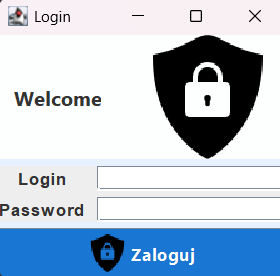
\includegraphics[width=0.4\textwidth]{figures/workApl/login_panel.png}
\caption{Panel logowania do systemu}
\label{fig:login_panel}
\end{figure}

\clearpage

\section*{Główny panel sekretariatu}

Na Rys. \ref{fig:mainpanel} widoczny jest główny panel sekretariatu. Panel ten jest centralnym miejscem zarządzania danymi w systemie. Wyświetla on tabelę ze wszystkimi zajęciami zapisanymi w bazie danych.

Użytkownik ma do dyspozycji przyciski:
\begin{itemize}
    \item \textbf{Dodaj} – otwiera formularz umożliwiający dodanie nowych zajęć,
    \item \textbf{Edytuj} – pozwala zmodyfikować zaznaczony rekord,
    \item \textbf{Usuń} – usuwa wybrane zajęcia z bazy,
    \item \textbf{Zastosuj filtry} – uruchamia filtrację danych,
    \item \textbf{Odśwież} – ładuje wszystkie dane ponownie.
\end{itemize}

Filtrowanie zajęć możliwe jest przez rozwijane listy, w których użytkownik może wybrać: salę, grupę lub typ zajęć. Dane prezentowane są w tabeli \texttt{JTable}, umieszczonej w kontenerze \texttt{JScrollPane}.

\begin{figure}[H]
\centering
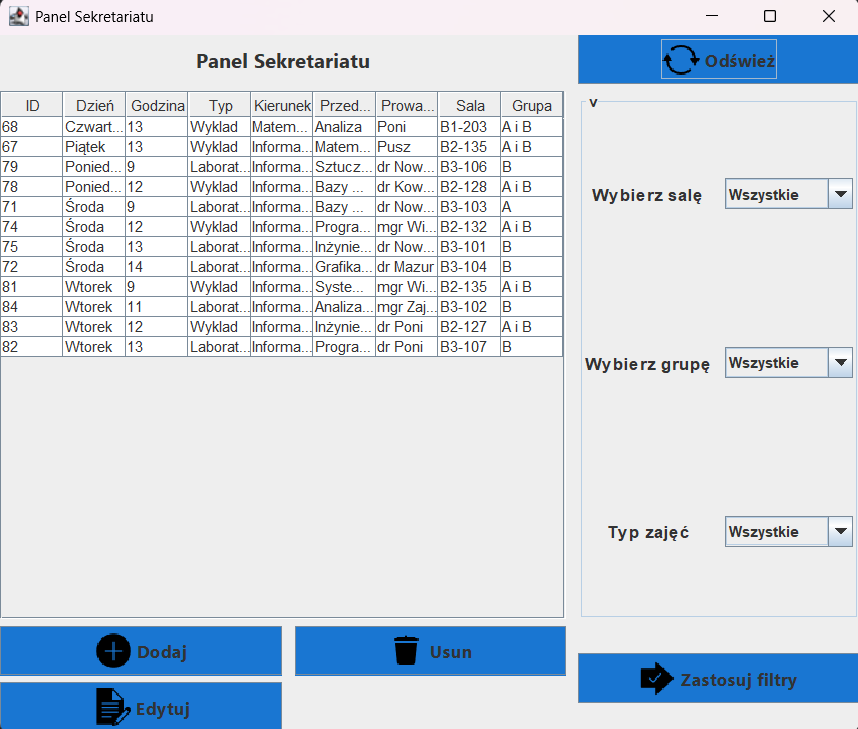
\includegraphics[width=0.9\textwidth]{figures/workApl/mainpanel.png}
\caption{Główny panel sekretariatu z listą zajęć i filtrowaniem}
\label{fig:mainpanel}
\end{figure}

\clearpage

\section*{Formularz dodawania zajęć typu Wykład}

Rysunek \ref{fig:add_wyklad} przedstawia panel umożliwiający dodawanie zajęć typu \textbf{Wykład}. Formularz ten zawiera pola tekstowe do uzupełnienia takich informacji jak kierunek studiów, nazwa przedmiotu, prowadzący, numer sali, dzień tygodnia oraz godzina.

Pola \texttt{Grupa 1} i \texttt{Grupa 2} są zablokowane, ponieważ wykład dotyczy wszystkich studentów danego kierunku niezależnie od przypisania do grupy.

\begin{figure}[H]
\centering
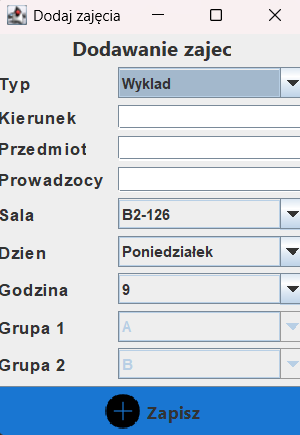
\includegraphics[width=0.45\textwidth]{figures/workApl/add_wyklad_panel.png}
\caption{Formularz dodawania zajęć typu Wykład}
\label{fig:add_wyklad}
\end{figure}

\clearpage

\section*{Formularz dodawania zajęć typu Laboratorium}

Na Rys. \ref{fig:add_lab} zaprezentowano formularz służący do dodawania zajęć typu \textbf{Laboratorium}. W tym przypadku możliwe jest przypisanie jednej grupy do zajęć – użytkownik wybiera ją w polu \texttt{Grupa 1}, natomiast \texttt{Grupa 2} pozostaje nieaktywne.

Formularz ten dostosowuje swoją funkcjonalność dynamicznie w zależności od wybranego typu zajęć. Przycisk \textbf{Zapisz} umożliwia dodanie danych po przejściu poprawnej walidacji.

\begin{figure}[H]
\centering
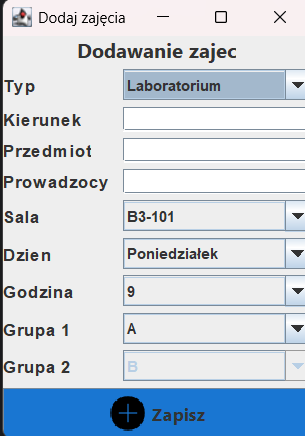
\includegraphics[width=0.45\textwidth]{figures/workApl/add_lab_panel.png}
\caption{Formularz dodawania zajęć typu Laboratorium}
\label{fig:add_lab}
\end{figure}

\clearpage

\section*{Formularz dodawania zajęć typu Projekt}

Jak przedstawiono na Rys. \ref{fig:add_projekt}, formularz ten umożliwia przypisanie dwóch grup do wspólnych zajęć typu \textbf{Projekt}. Dane te są zapisywane zarówno w tabeli \texttt{zajecia}, jak i w powiązanej tabeli \texttt{projekty}.

Użytkownik musi podać wszystkie wymagane informacje: kierunek, przedmiot, prowadzący, sala, dzień i godzina zajęć, oraz przypisać obie grupy projektowe. System weryfikuje poprawność danych oraz sprawdza potencjalne konflikty terminów przed zapisaniem rekordu.

\begin{figure}[H]
\centering
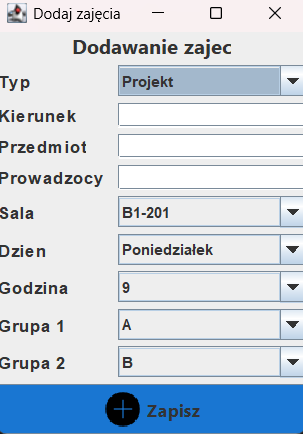
\includegraphics[width=0.45\textwidth]{figures/workApl/add_projekt_panel.png}
\caption{Formularz dodawania zajęć typu Projekt}
\label{fig:add_projekt}
\end{figure}

\clearpage

\section*{Formularz edycji zajęć}

Rys. \ref{fig:edit_panel} prezentuje panel edycji zajęć. Użytkownik może zaznaczyć rekord z tabeli głównego panelu i przejść do jego modyfikacji. Wszystkie dane z wybranego wiersza są automatycznie załadowane do formularza.

Po zakończeniu edycji wystarczy kliknąć przycisk \textbf{Zapisz}, aby zapisać zmiany w bazie danych. Formularz umożliwia edycję dowolnego typu zajęć — również typu \texttt{Projekt} i \texttt{Laboratorium}, przy czym zachowane są te same zasady walidacji co podczas dodawania.

\begin{figure}[H]
\centering
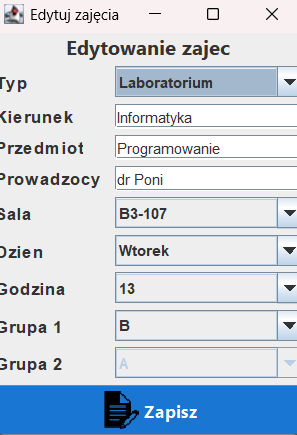
\includegraphics[width=0.45\textwidth]{figures/workApl/edit_panel.png}
\caption{Formularz edycji istniejących zajęć}
\label{fig:edit_panel}
\end{figure}

\subsection{Baza danych}

Dane przechowywane są w relacyjnej bazie danych \textbf{PostgreSQL}, w ramach schematu \texttt{public} bazy \texttt{javabase}. System korzysta z następujących tabel:

\begin{itemize}
    \item \texttt{zajecia} – główna tabela przechowująca dane o wszystkich zajęciach:
    \begin{itemize}
        \item \texttt{id}, \texttt{typ}, \texttt{kierunek}, \texttt{przedmiot}, \texttt{prowadzacy}, \texttt{sala}, \texttt{dzien}, \texttt{godzina}, \texttt{grupa1}, \texttt{grupa2}.
    \end{itemize}

    \item \texttt{projekty} – zawiera przypisanie dwóch grup do zajęć typu \texttt{Projekt}:
    \begin{itemize}
        \item \texttt{zajecia\_id}, \texttt{grupa1}, \texttt{grupa2}.
    \end{itemize}

    \item \texttt{laboratoria} – przechowuje numer grupy przypisanej do zajęć typu \texttt{Laboratorium}:
    \begin{itemize}
        \item \texttt{zajecia\_id}, \texttt{nr\_grupy}.
    \end{itemize}

    \item \texttt{uzytkownicy} – tabela logowania przechowująca dane uwierzytelniające użytkowników:
    \begin{itemize}
        \item \texttt{id}, \texttt{login}, \texttt{haslo}.
    \end{itemize}
\end{itemize}

Tabele są powiązane logicznie przez kolumnę \texttt{zajecia\_id}, a dane zabezpieczone są poprzez ograniczenia integralności oraz indeksy. Struktura została zaprojektowana tak, aby umożliwiać wygodne wykonywanie operacji CRUD i filtrowania.

\subsection{Diagram Baza Danych}

\begin{figure}[H]
    \centering
    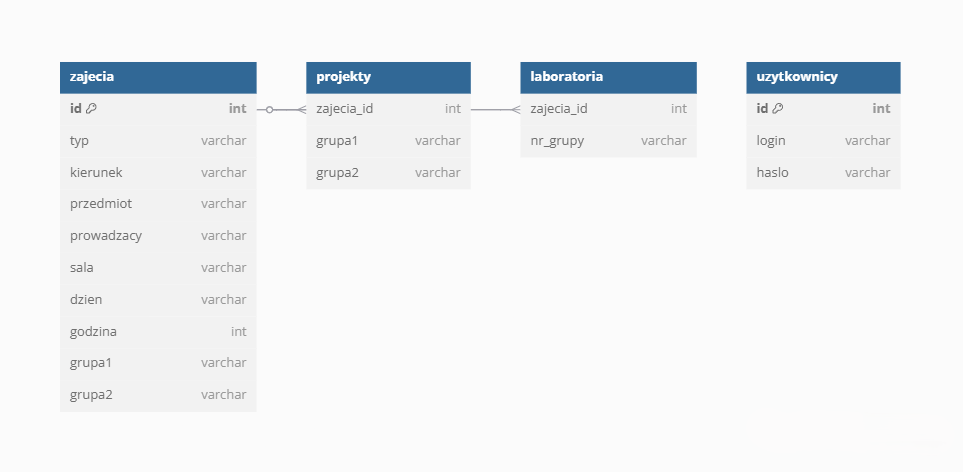
\includegraphics[width=0.85\textwidth]{figures/diagramDB.png}
    \caption{Diagram relacyjny bazy danych systemu}
    \label{fig:diagram-db}
\end{figure}
\section{Interfejs użytkownika}

Interfejs został wykonany w technologii \textbf{Swing}. Główne okna aplikacji to:

\begin{itemize}
    \item \textbf{Ekran logowania} – umożliwia dostęp tylko zalogowanym użytkownikom;
    \item \textbf{Panel sekretariatu} – pozwala na przeglądanie i zarządzanie zajęciami;
    \item \textbf{Formularz dodawania zajęć} – umożliwia wprowadzenie nowych zajęć;
    \item \textbf{Formularz edycji zajęć} – pozwala na modyfikację istniejących rekordów.
\end{itemize}

\section{Walidacja i błędy}

System zawiera zabezpieczenia:

\begin{itemize}
    \item Sprawdzanie dostępności sali w wybranym dniu i godzinie;
    \item Sprawdzanie, czy dana grupa nie ma już zajęć w tym czasie;
    \item Obsługa wyjątków SQL i wyświetlanie komunikatów błędów użytkownikowi.
\end{itemize}

\section{Szczegółowy opis komponentów GUI}

\subsection {Formularz Dodawania Zajęć (DodajZajeciaPanel)}

\begin{itemize}
    \item \textbf{Cel:} Dodawanie nowych rekordów zajęć do bazy danych.
    \item \textbf{Elementy:}
    \begin{itemize}
        \item \texttt{JComboBox} – typ zajęć (np. Wykład, Laboratorium, Projekt);
        \item \texttt{JTextField} – kierunek, przedmiot, prowadzący, sala, godzina, grupa1, grupa2;
        \item \texttt{JComboBox} – dzień tygodnia;
        \item \texttt{JButton} – „Zapisz” — zapisuje dane do bazy danych.
    \end{itemize}
    \item \textbf{Uwagi:} Interfejs zawiera etykiety (\texttt{JLabel}) przypisane do każdego pola. Formularz obsługuje walidację przed zapisem zajęć.
\end{itemize}

\subsection {Formularz Edytowania Zajęć (EdytujZajeciaPanel)}

\begin{itemize}
    \item \textbf{Cel:} Edytowanie istniejących danych zajęć.
    \item \textbf{Elementy:} Te same co w \texttt{DodajZajeciaPanel}, jednak służą do aktualizacji danych:
    \begin{itemize}
        \item Pola są wstępnie wypełnione danymi z wybranego rekordu;
        \item \texttt{JButton} – „Zapisz” — aktualizuje dane w bazie.
    \end{itemize}
    \item \textbf{Uwagi:} Pola są edytowalne i automatycznie uzupełniane na podstawie danych wybranych z tabeli.
\end{itemize}

\subsection {Formularz Logowania (Login)}

\begin{itemize}
    \item \textbf{Cel:} Autoryzacja użytkownika w systemie.
    \item \textbf{Elementy:}
    \begin{itemize}
        \item \texttt{JTextField} – login;
        \item \texttt{JPasswordField} – hasło;
        \item \texttt{JButton} – „Zaloguj” — weryfikuje dane logowania.
    \end{itemize}
    \item \textbf{Uwagi:} Prosty, nowoczesny wygląd z ikoną kłódki; Zabezpieczenie dostępu do aplikacji.
\end{itemize}

\subsection {Panel Sekretariatu (SekretariatPanel)}

\begin{itemize}
    \item \textbf{Cel:} Zarządzanie zajęciami (CRUD).
    \item \textbf{Elementy:}
    \begin{itemize}
        \item \texttt{JTable} – wyświetlanie listy zajęć;
        \item \texttt{JComboBox} – filtrowanie po sali, grupie, typie zajęć;
        \item \texttt{JButton} – „Dodaj”, „Usuń”, „Edytuj”, „Zastosuj filtry”, „Odśwież”;
        \item \texttt{JScrollPane} – przewijana tabela;
        \item \texttt{JLabel} – etykiety opisowe.
    \end{itemize}
    \item \textbf{Uwagi:} Obsługuje filtrowanie i pełną obsługę CRUD; główny ekran zarządzania.
\end{itemize}

\clearpage
\section{Diagram komponentów GUI i zależności}

Diagram przedstawiony na Rys. \ref{fig:diagram-gui} ilustruje architekturę aplikacji oraz przepływ zależności pomiędzy jej głównymi komponentami. Aplikacja została zaprojektowana zgodnie z podejściem warstwowym (ang. layered architecture), które oddziela logikę GUI, model danych, logikę dostępu do danych (DAO) oraz warstwę połączenia z bazą danych.

\begin{itemize}
    \item Komponenty pakietu \texttt{gui} odpowiadają za graficzny interfejs użytkownika: \texttt{SekretariatPanel}, \texttt{DodajZajeciaPanel}, \texttt{EdytujZajeciaPanel}, \texttt{Login}.
    \item Komponenty modelu (\texttt{Zajecia}, \texttt{Wykład}, \texttt{Projekt}, \texttt{Laboratorium}) reprezentują dane przekazywane między warstwami.
    \item Pakiet \texttt{dao} zawiera klasy \texttt{ZajeciaDAO} oraz \texttt{LoginDAO}, odpowiedzialne za dostęp do bazy danych poprzez odpowiednie metody (np. \texttt{getAllZajecia()}, \texttt{addZajecia()}, \texttt{login()}).
    \item Warstwa \texttt{database} odpowiada za ustanowienie połączenia z bazą danych — klasę \texttt{DatabaseConnection}.
\end{itemize}

Zależności między komponentami są jednokierunkowe, co sprzyja testowalności i rozszerzalności systemu. GUI komunikuje się wyłącznie z DAO, które obsługuje logikę zapisu i odczytu danych z relacyjnej bazy danych PostgreSQL.

\begin{figure}[H]
    \centering
    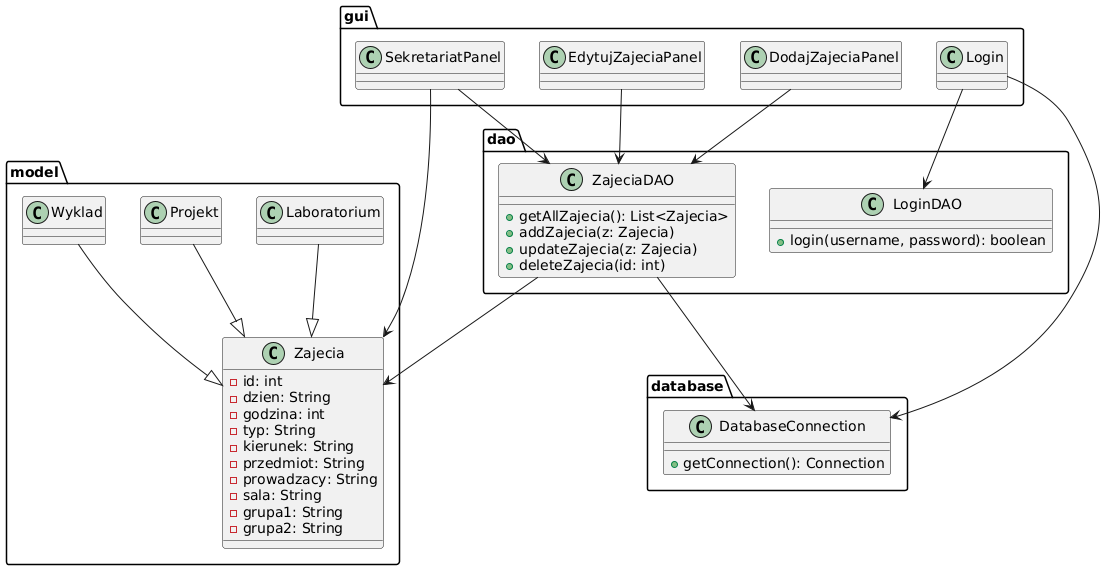
\includegraphics[width=0.95\textwidth]{figures/diagram.png}
    \caption{Zależności pomiędzy komponentami GUI, modelem danych i warstwą DAO}
    \label{fig:diagram-gui}
\end{figure}


% Wyłączenie działania `ulem` na czas bibliografii
\renewcommand{\emph}[1]{\textit{#1}}
% Bibliografia
% Dodanie bibliografi do spisu treści
\addcontentsline{toc}{section}{\textbf{Bibliografia}}
\bibliographystyle{plain}
\bibliography{bibliografia}

% Przywrócenie działania `ulem`
\renewcommand{\emph}[1]{\uline{#1}}

\clearpage
% Dodanie spisu rysunków do spisu treści
\addcontentsline{toc}{section}{\textbf{Spis rysunków}}
\listoffigures
\clearpage

% Dodanie spisu tabel do spisu treści
\addcontentsline{toc}{section}{\textbf{Spis tabel}}
\listoftables
\clearpage


\clearpage

% Dodanie spisu listingow do spisu treści
\addcontentsline{toc}{section}{\textbf{Spis listingów}}
\lstlistoflistings
\clearpage


% \appendix
\chapter*{}
\label{cha:statement-A}
\makeatletter
\addcontentsline{toc}{section}{\textbf{Oświadczenie studenta o samodzielności pracy}}

\noindent
\begin{flushright}
    \begin{minipage}[!h]{10cm}
        Załącznik nr 2 do Zarządzenia nr 228/2021 Rektora Uniwersytetu Rzeszowskiego z dnia 1 grudnia 2021 roku w sprawie ustalenia procedury antyplagiatowej w Uniwersytecie Rzeszowskim
    \end{minipage}
\end{flushright}

\begin{center}
    \vspace*{10mm}
    \noindent  {\textbf{OŚWIADCZENIE STUDENTA O SAMODZIELNOŚCI PRACY} }
    \vspace*{10mm}
\end{center}

\noindent
\dotuline{\hspace{1.3cm}\@author\hspace{1.3cm}}\\ % Linia pozioma
{\small Imię (imiona) i nazwisko studenta }\\

\noindent \@faculty\\

\noindent \dotuline{\hspace{1.4cm}\@degreeprogramme \hspace{1.4cm}}\\
{\small Nazwa kierunku} \\

\noindent \dotuline{\hspace{1.8cm}\@noAlbum\hspace{1.9cm}}\\
{\small Numer albumu}

\begin{enumerate}
    \item Oświadczam, że moja praca projektowa pt.: \@titlePL
          \begin{enumerate}[label=\arabic*)]
              \item została przygotowana przeze mnie samodzielnie,
              \item nie narusza praw autorskich w rozumieniu ustawy z dnia 4 lutego 1994 roku o prawie autorskim i prawach pokrewnych (t.j. Dz.U. z 2021 r., poz. 1062) oraz dóbr osobistych chronionych prawem cywilnym,
              \item nie zawiera danych i informacji, które uzyskałem/am w sposób niedozwolony,
              \item nie była podstawą otrzymania oceny z innego przedmiotu na uczelni wyższej ani mnie, ani innej osobie.
          \end{enumerate}
    \item Jednocześnie wyrażam zgodę na udostępnienie mojej pracy projektowej do celów naukowo--badawczych z poszanowaniem przepisów ustawy o prawie autorskim i prawach pokrewnych.
\end{enumerate}


\vspace*{10mm}

\noindent
\underline{\hspace{6cm}} \hfill \underline{\hspace{6cm}} \\ % Puste miejsce na miejscowość, data oraz podpis
\hspace*{13mm}(miejscowość, data)  \hspace*{63mm}(czytelny podpis studenta)
\vspace*{10mm}

\vfill
\noindent


\end{document}
